\documentclass{article}

\usepackage[english]{babel}

\usepackage[letterpaper,top=2cm,bottom=2cm,left=3cm,right=3cm,marginparwidth=1.75cm]{geometry}

% Useful packages
\usepackage{amsmath}
\usepackage{amssymb}
\usepackage{graphicx}
\usepackage{mathtools}
\usepackage{tikz}
\usepackage[colorlinks=true, allcolors=blue]{hyperref}
\usepackage{xcolor}
\usepackage{colortbl}
\usepackage{booktabs}
\usepackage{tikz}
\usepackage{tcolorbox}
\usetikzlibrary{positioning, arrows.meta}

\newcommand{\Fp}{\mathbb F_p}
\newcommand{\Fq}{\mathbb F_q}
\newcommand{\Pol}{T}

\title{Whirlaway: multilinear PIOP for AIR}
\author{Thomas Coratger, Tom Wambsgans}
\date{}
\begin{document}
\maketitle

\section{Introduction}

AIR (Algebraic Intermediate Representation) is a common arithmetization standard is the context of (ZK)-SNARK (Succint Non-Interactive Argument of Knowledge, potentially Zero-Knowledge). Traditionally, AIR constraints were proven using a univariate PIOP (Polynomial Interactive Oracle Proof), as explained in the EthStark paper \cite{eth_stark}.
Whirlaway is a simple multilinear PIOP, proving AIR constraints, focusing on lightweight proofs. 

The multilinear framework has two main advantages compared to classical approaches. First, it enables encoding and committing the entire AIR execution trace as a single multilinear polynomial, instead of encoding each table column as a separate low-degree univariate polynomial. In many modern proof systems, the correctness of a computation is expressed through multiple tables, each capturing specific CPU instructions (in the context of zkVMs) or constraints. To enable efficient verification, the prover encodes the columns of these tables as low-degree polynomials and commits to them using a polynomial commitment scheme. However, this design introduces a caveat: the prover must commit to and provide evaluation proofs for each polynomial separately, and the verifier must process and check each of these commitments individually. As the number of columns grows, the verifier’s workload and the overall proof size scale linearly, which can significantly impact efficiency.

Second, the multilinear approach allows proving the validity of AIR constraints using the sumcheck protocol, which removes the need for a quotient polynomial. In the classical univariate approach, AIR constraints are bundled into a single vanishing condition, and the prover must construct and commit to a quotient polynomial that encodes the division of the constraint polynomial by the vanishing polynomial of the domain. The opening proof for the committed quotient polynomial again increases the proof size. From the prover perspective, using a quotient polynomial coupled with a FRI based PCS (superlinear time) may also be slower than the sumcheck (linear time) algorithm


Paired with the recent WHIR Polynomial Commitment Scheme \cite{whir}, we obtain a hash-based SNARK, plausibly post quantum, with small proof size (on the order of 128 KiB), and promising proving speed (an experimental implementation reached one million Poseidon2 permutations proven per second, on the KoalaBear field, with 128 bits of security, on a RTX 4090).

An initial implementation can be found \href{https://github.com/TomWambsgans/Whirlaway}{here}.

\section{Definitions and notations}

\subsection{Multilinear framework}

\subsubsection{Multilinear polynomial}

A multilinear polynomial over variables $X_1, \dots, X_k$ is a multivariate polynomial where each variable appears with degree at most one. Formally, it can be written as:
$$
    P(X_1, \dots, X_k) = \sum_{S \subseteq [k]} c_S \prod_{i \in S} X_i,
$$
where each $c_S \in \Fp$ is a coefficient, and the sum ranges over all subsets $S$ of ${1, \dots, k}$. For example, over two variables $X, Y$, the polynomial $3 + 2X + 5Y + 7XY$ is multilinear, but $X^2$ or $Y^3$ are not.

A multilinear polynomial is uniquely identified by its evaluation on the boolean hypercube:

$$
    P(X_1, \dots, X_k) = \sum_{b \in \{0, 1\}^k} eq((X_1, \dots, X_k), b) \cdot P(b)
$$


\subsubsection{Multilinear extension}



Given a function $f: \{0,1\}^n \to \Fp$, its multilinear extension $\widehat{f}: \Fp^n \to \Fp$ is the unique multilinear polynomial over $n$ variables that agrees with $f$ on all Boolean inputs. Explicitly, it can be written as:

$$
\widehat{f}(x) = \sum_{b \in \{0,1\}^n} f(b) \cdot eq(b, x)
$$

This extension allows evaluating the function not just at Boolean points, but at any point $x \in \Fp^n$.


\subsection{Notations}

\begin{itemize}
    \item $log$ is always in base 2
    \item $[i]_2$: big-endian bit decomposition of an integer $i$
    \item $eq(x, y) := \prod_{i = 1}^{n} (x_i y_i + (1 - x_i) (1 - y_i))$, for $x$ and $y$ in $\mathbb F^n$. This "equality multilinear polynomial" verifies: $eq(x, y) = 1$ if $x = y$, $0$ otherwise, for $x$ and $y$ both sampled on the hypercube $\{0, 1\}^n$.
    \item $\Fp$: base field, typically KoalaBear ($p = 2^{31} - 2^{24} + 1$), or BabyBear ($p = 2^{31} - 2^{27} + 1$)
    \item $\Fq$: extension field ($q = p^\kappa$)
    \item $M$ $(\text{resp. } M')$: number of columns (resp. non-preprocessed columns) in the AIR table
    \item $m$ $(\text{resp. } m')$: smallest integer such that $2^m \geq M$ (resp. $2^{m'} \geq M'$)
    \item $N = 2^n$: number of rows in the AIR table
    \item $h_1, \dots, h_u$: transition constraints
    \item $H$: batched constraint ($H := \sum_{i=0}^{u-1} h_i \alpha^i $)
    \item $\Pol$: multilinear polynomial in $\Fp$ encoding all the (non-preprocessed) columns, with $n + m'$ variables
\end{itemize}

\section{AIR Arithmetization}

\subsection{Description}

In the AIR arithmetization, the witness consists of a list of $M$ columns $c_0, \dots, c_{M-1}$ (forming the AIR table). Each column contains $N = 2^n$ elements in $\Fp$ (without loss of generality, we use a power-of-two domain). The goal of the prover is to convince the verifier that the table respects a set of $u$ transition constraints $h_0, \dots, h_{u-1}$. Each constraint $h$ is a polynomial in $2 M$ variables, which is respected if for all rows $r \in \{0, \dots, N-2\}$: 

$$h(c_0[r], \dots, c_{M-1}[r], c_0[r+1], \dots, c_{M-1}[r+1]) = 0$$

\subsection{Preprocessed columns}

Traditional AIR systems allow the verifier to fix certain cells in the table (see "boundary conditions" \href{https://aszepieniec.github.io/stark-anatomy/stark}{here}). For technical reasons, we use a slightly different approach: we allow the verifier to fix certain columns, potentially sparse (called "preprocessed columns"). The work of the verifier associated to each preprocessed column is proportional to its number of nonzero rows. We denote by $c_0, \dots, c_{M'-1}$ the non-preprocessed columns and $c_{M'}, \dots, c_{M-1}$ the preprocessed ones.

\subsection{Example: Fibonacci sequence}


In general, each constraint $h_i$ is a polynomial relation over the current and next rows of the table. We use the notation $X_j^{\text{up}}$ to refer to the value of column $c_j$ at row $r$ (the “upper” row), and $X_j^{\text{down}}$ to refer to its value at row $r + 1$ (the “lower” row). These variables appear as inputs to the $h_i$ constraints, which together enforce the correct behavior across the table. Each constraint has the form:
$$
h_i(\underbrace{X_0^{\text{up}}, \dots, X_{M-1}^{\text{up}}}_{\text{Upper row columns}}, \underbrace{X_0^{\text{down}}, \dots, X_{M-1}^{\text{down}}}_{\text{Lower row columns}}) = \text{some constraint}
$$
where:
\begin{itemize}
    \item $X_j^{\text{up}} = c_j[r]$ is the value of column $c_j$ at row $r$
    \item $X_j^{\text{down}} = c_j[r + 1]$ is the value of column $c_j$ at row $r + 1$
\end{itemize}

Let's say the prover wants to convince the verifier that the $N$-th values of the Fibonacci sequence equals $F_N$. We use $M = 4$ columns, as illustrated in Figure~\ref{fig:fibonacci_air}:

\begin{itemize}
    \item The first $M' = 2$ columns $c_0$ and $c_1$ contain the values of the Fibonacci sequence, which is guaranteed by the constraints:

\begin{itemize}
    \item $h_0$ constraint ensures that the next $c_1$ value equals the sum of the current $c_0$ and $c_1$ values, i.e., $F_{r+2} = F_r + F_{r+1}$:
    
    $$h_0(X_0^{\text{up}}, X_1^{\text{up}}, -, -, -, X_1^{\text{down}}, -, -) = X_1^{\text{down}} - (X_0^{\text{up}} + X_1^{\text{up}})$$
    \item $h_1$ constraint shifts the sequence forward, ensuring that the next $c_0$ value equals the current $c_1$ value:
    
    $$h_1(-, X_1^{\text{up}}, -, -, X_0^{\text{down}}, -, -, -) = X_0^{\text{down}} - X_1^{\text{up}}$$
\end{itemize}

 \item The last two columns $c_2$ and $c_3$ are "preprocessed": their content is enforced by the verifier. In our case we set $c_2 = [1, 0, \dots, 0]$ to act as a selector for the initial row and $c_3 = [0, \dots, 0, 1]$ as a selector for the final row. We finally use the following constraints, to ensure that the 2 initial values of the sequence are correct ($0$ and $1$), and that the final value equals $F_N$:

 \begin{itemize}
    \item $h_2$ ensures that $c_0=0$ when $c_2 \neq 0$ (which only occurs at the first row):
    $$h_2(X_0^{\text{up}}, -, X_2^{\text{up}}, -, -, -, -, -) =   X_2^{\text{up}} \cdot X_0^{\text{up}}$$
    
    \item $h_3$ ensures $c_1 = 1$ when $c_2 \neq 0$ (only at the first row).
    
    $$h_3(-, X_1^{\text{up}}, X_2^{\text{up}}, -, -, -, -, -) =  X_2^{\text{up}} \cdot (X_1^{\text{up}} - 1) $$ 

% (When the selector $c_2 \neq 0$ (which turns out to be the case at the initial row), we necessarily have $c_0 = 0$ and $c_1 = 1$)

 \item $h_4$ ensures $c_0 = F_N$ when $c_3 \neq 0$ (only at the last row).
 
 $$h_4(X_0^{\text{up}}, -, -, X_3^{\text{up}}, -, -, -, -) = X_3^{\text{up}} \cdot (X_0^{\text{up}} - F_n)$$ 

% (When the selector $c_3 \neq 0$ (which turns out to be the case at the final row), we necessarily have $c_0 = F_n$)

\end{itemize}

Note that $c_2$ and $c_3$ are sparse, both contain only one non-zero index. As a consequence, they have a negligible impact on the verification time.

 \end{itemize}


\begin{figure}[h!]
\centering
\begin{tabular}{ccccc}
\toprule
Row & $c_0$ & $c_1$ & $c_2$ (preproc.) & $c_3$ (preproc.) \\
\midrule
0 & \cellcolor{blue!10}0 & \cellcolor{blue!10}1 & \cellcolor{orange!10}1 & \cellcolor{orange!10}0 \\
1 & \cellcolor{blue!10}1 & \cellcolor{blue!10}1 & \cellcolor{orange!10}0 & \cellcolor{orange!10}0 \\
2 & \cellcolor{blue!10}1 & \cellcolor{blue!10}2 & \cellcolor{orange!10}0 & \cellcolor{orange!10}0 \\
$\vdots$ & $\vdots$ & $\vdots$ & $\vdots$ & $\vdots$ \\
N-1 & \cellcolor{blue!10}$F_N$ & \cellcolor{blue!10}$F_{N+1}$ & \cellcolor{orange!10}0 & \cellcolor{orange!10}1 \\
\bottomrule
\end{tabular}

\vspace{1em}
\caption{Fibonacci sequence AIR table layout with preprocessed selectors}
\label{fig:fibonacci_air}
\end{figure}

\section{Proving system}

\subsection{{Commitment}}

Contrary to most of the STARK systems, which use a univariate Polynomial Commitment Scheme (PCS), like FRI or KZG, we use instead a multilinear one. 



The entire AIR table is encoded and committed as a single multilinear polynomial $\Pol$ (except for the preprocessed columns, which are not committed). $\Pol$ has $n + m'$ variables, where $n = \log N = \log \text{(number of rows)}$ and $m' = \left\lceil  \log M' \right\rceil = \left\lceil  \log \text{(number of non-preprocessed columns)} \right\rceil$. $\Pol$ is defined by its evaluations over the boolean hypercube: for every (non-preprocessed) column index $i$ ($0 \leq i < M'$) and for every row index $r$ ($0 \leq r < N$): 

$$\Pol([i]_2 [r]_2) := c_{i}[r],$$

where:
\begin{itemize}
    \item $[i]_2$ is the big-endian bit decomposition of $i$ into $m'$ bits (where $m' = \lceil \log M' \rceil$)
    \item $[r]_2$ is the big-endian bit decomposition of $r$ into $n$ bits (where $n = \log N$)
    \item $[i]_2 [r]_2$ represents concatenated $m' + n$ bits
\end{itemize}

For example, if $M' = 20$, $N = 128$, $i = 3$, and $r = 33$, we have:
$$
[i]_2 = 00011, \quad [r]_2 = 0100001, \quad [i]_2 [r]_2 = 00011 \, | \, 0100001.
$$

This means that $\Pol$ evaluates at the point corresponding to these bits to give:
$$
\Pol(00011 \, | \, 0100001) = c_3[33]
$$

% Where $[i]_2$ and $[r]_2$ are the corresponding bit decomposition (big-endian) of $i$ and $r$ (e.g. $M' = 20, N = 128, i = 3, r = 33, [i]_2[r]_2 = (00011 | 0100001)$).

The undefined evaluations (for indices $M' \leq i < 2^{m'}$) are irrelevant and can be set to zero.

% Note that the coefficients of $\Pol$ are in the base field $\Fp$. The random evaluation point at which $\Pol$ will be queried later by the verifier is in the extension field $\Fq$ (for soundness). 

Note that the coefficients of $\Pol$ are in the base field $\Fp$, while the verifier will later query $\Pol$ at a random evaluation point drawn from the extension field $\Fq$. Querying over the larger extension field is important for soundness because it reduces the prover's chance of successfully cheating: the Schwartz-Zippel lemma guarantees that a nonzero polynomial will evaluate to zero at a random point with probability at most $\deg / |\Fq|$, and using a larger field strengthens this bound.

One solution is to embed $\Pol$ into the extension field $\Fq$ before committing to it, but this create overhead.
Section~\ref{embedding_overhead} describes a simple and efficient approach to avoid this "embedding overhead" with WHIR.

\subsection{Batching the constraints}

After receiving the commitment to $\Pol$, the verifier sends a random scalar $\alpha \in \Fq$ to the prover. Up to a small soundness error, we can replace the $u$ transition constraints by a single one: 

$$H := \sum_{i=0}^{u-1} h_i \alpha^i $$

The batched constraint $H$ is a single combined polynomial that aggregates all the individual transition constraints $h_0, \dots, h_{u-1}$. Instead of checking each $h_i$ separately, we check $H$ once, which compresses the verification work while preserving soundness.

\subsection{Zerocheck} \label{zerocheck}

The main argument comes from \cite{ccs} (see also \cite{simple_multivariate_AIR}). For each column $c$, we define two multilinear polynomials over $n$ variables:
\begin{itemize}
    \item The shifted copy $c^{\text{up}}$,
    \item The forward-shifted copy $c^{\text{down}}$.
\end{itemize}

Specifically, as illustrated in Figure~\ref{fig:zerocheck_mappings_n4}:

\begin{equation}
\begin{aligned}
c^{\text{up}}([r]_2) &= 
\begin{cases}
c[r] & \text{if } r \in \{0, \dots, N - 2\} \\
c[N - 2] & \text{if } r = N - 1
\end{cases} \\
c^{\text{down}}([r]_2) &= 
\begin{cases}
c[r + 1] & \text{if } r \in \{0, \dots, N - 2\} \\
c[N - 1] & \text{if } r = N - 1
\end{cases}
\end{aligned}
\end{equation}


\begin{figure}[h!]
\centering
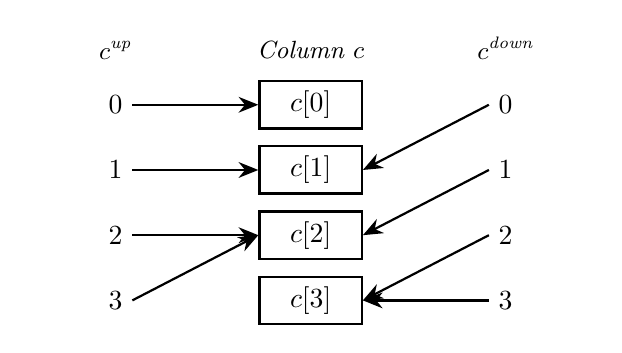
\begin{tikzpicture}[
    node distance=0.2cm and 1.6cm, % Further reduced y-distance to 0.2cm
    cnode/.style={draw, rectangle, minimum height=0.6cm, minimum width=1.3cm, anchor=center, thick}, % Reduced height
    rnode/.style={minimum height=0.6cm, anchor=center, font=\ttfamily}, % Reduced height
    arrowstyle/.style={-{Stealth[length=2.5mm, width=2mm]}, thick},
    labelstyle/.style={font=\small\itshape}
]

\node[cnode] (c0) {$c[0]$};
\node[cnode] (c1) [below=of c0] {$c[1]$};
\node[cnode] (c2) [below=of c1] {$c[2]$};
\node[cnode] (c3) [below=of c2] {$c[3]$};
\node[labelstyle, above=0.15cm of c0] {Column $c$}; % Slightly reduced space

% Inputs r for c^{up} (left)
\node[rnode] (r0_up) [left=of c0] {$0$};
\node[rnode] (r1_up) [left=of c1] {$1$};
\node[rnode] (r2_up) [left=of c2] {$2$};
\node[rnode] (r3_up) [left=of c3] {$3$};
\node[labelstyle, text width=2cm, align=center, above=0.15cm of r0_up] {$c^{\text{up}}$}; % Slightly reduced space

\draw[arrowstyle] (r0_up.east) -- (c0.west);
\draw[arrowstyle] (r1_up.east) -- (c1.west);
\draw[arrowstyle] (r2_up.east) -- (c2.west);
\draw[arrowstyle] (r3_up.east) -- (c2.west);

% Inputs r for c^{down} (right)
\node[rnode] (r0_down) [right=of c0] {$0$};
\node[rnode] (r1_down) [right=of c1] {$1$};
\node[rnode] (r2_down) [right=of c2] {$2$};
\node[rnode] (r3_down) [right=of c3] {$3$};
\node[labelstyle, text width=2cm, align=center, above=0.15cm of r0_down] {$c^{\text{down}}$}; % Slightly reduced space

\draw[arrowstyle] (r0_down.west) -- (c1.east);
\draw[arrowstyle] (r1_down.west) -- (c2.east);
\draw[arrowstyle] (r2_down.west) -- (c3.east);
\draw[arrowstyle] (r3_down.west) -- (c3.east);

\end{tikzpicture}
\caption{Visualization of $c^{\text{up}}$ and $c^{\text{down}}$ for $N=4$.}
\label{fig:zerocheck_mappings_n4}
\end{figure}

The batched constraint $H$ is respected on the table if and only if:

$$\begin{gathered}
\forall r \in \{0, \dots, N-2\}, \hspace{2mm} H(c_0[r], \dots, c_{M-1}[r], c_0[r+1], \dots, c_{M-1}[r+1]) = 0 \\
\Leftrightarrow\\
\forall r \in \{0, \dots, N-1\}, \hspace{2mm} H(c_0^{\text{up}}([r]_2), \dots, c_{M-1}^{\text{up}}([r]_2), c_0^{\text{down}}([r]_2), \dots, c_{M-1}^{\text{down}}([r]_2)) = 0
\end{gathered}$$

The last equality can be proven using a zerocheck (see \cite{hyperplonk}), assuming the verifier has oracle access to $c_0^{\text{up}}, \dots, c_{M-1}^{\text{up}}$ and $ c_0^{\text{down}}, \dots, c_{M-1}^{\text{down}}$, which will be addressed in Section~\ref{shifted_mle}. The zerocheck is performed as follows:

\begin{enumerate}
    \item The verifier sends a random vector $r \in \Fq^n$,
    \item Prover and verifier run the sumcheck protocol to prove that:
    $$ \sum_{b \in \{0, 1\}^n} eq(b, r) \cdot H(c_0^{\text{up}}(b), \dots, c_{M-1}^{\text{up}}(b), c_0^{\text{down}}(b), \dots, c_{M-1}^{\text{down}}(b)) = 0 $$
    \item At each round $i$ of the sumcheck, the verifier sends a random challenge $\beta_i \in \Fq$. At the end of the final round, the verifier needs to evaluate the expression inside the sum above for $b \xleftarrow{} \beta = (\beta_1, \dots, \beta_n)$.
    \begin{itemize}
        \item The factor $eq(\beta, r)$ can be computed directly by the verifier.
        \item For the remaining part, the prover provides the claimed evaluations (how the verifier checks the correctness of these values will be detailed in Section~\ref{shifted_mle}.):
        \begin{equation*}
            c_0^{\text{up}}(\beta), \dots, c_{M-1}^{\text{up}}(\beta), \quad c_0^{\text{down}}(\beta), \dots, c_{M-1}^{\text{down}}(\beta)
        \end{equation*}
        Given these $2M$ values, the verifier can finally evaluate $H$, which concludes the zerocheck.
    \end{itemize}
\end{enumerate}

\subsection{Oracle access to \texorpdfstring{$\textbf{\textit{c}}^{\text{up}}$}{} and \texorpdfstring{$\textbf{\textit{c}}^{\text{down}}$}{}}\label{shifted_mle}

In Section~\ref{zerocheck}, for each column $c_i$, the prover has sent two values: $\text{claim}^\text{up}_i$ and $\text{claim}^\text{down}_i$ respectively equal to $c_i^{\text{up}}(\beta)$ and $c_i^{\text{down}}(\beta)$ in the honest case. It is now time to prove the correctness of these $2M$ evaluations.

First, the verifier sends a random challenge $\gamma \in \Fq$. Except with small soundness error, the $2M$ claims can be reduced to the following:

\begin{equation}\label{eq1}
    \sum_{i = 0}^{M-1} (\gamma^i \cdot \text{claim}^\text{up}_i + \gamma^{i+M} \cdot \text{claim}^\text{down}_i) \stackrel{?}{=} \sum_{i = 0}^{M-1} (\gamma^i \cdot c_i^{\text{up}}(\beta) + \gamma^{i+M} \cdot c_i^{\text{down}}(\beta))
\end{equation}

\begin{itemize}
    \item Left-hand side: the verifier can compute it directly using the claimed values.
    \item Right-hand side: we need explicit formulas for $c_i^{\text{up}}$ and $c_i^{\text{down}}$ in terms of the multilinear extension of the the corresponding column $c_i$:
\end{itemize}


\subsubsection{\texorpdfstring{Expression of $\textbf{\textit{c}}^{\text{up}}$}{}} \label{shifted_mle_up}

For every column $c$, for every $r \in \Fq^n$, we have:
\begin{equation*}
    \begin{aligned}
        c^{\text{up}}(r) &=  \sum_{b \in \{0, 1\}^n}  \text{shift}^{\text{up}}(r, b) \cdot \widehat{c}(b) \\
        &=  \sum_{b \in \{0, 1\}^n} \left[\overbrace{eq(b, r) \cdot (1 - eq(r, (\underbrace{1, \dots, 1}_{n \text{ times}})))}^{\text{picks $c[r]$ when $r \neq N_1$ (i.e. before the last row)}} + \overbrace{eq((r, b), (\underbrace{1, \dots, 1}_{2n - 1 \text{ times}}, 0))}^{\text{picks $c[N - 2]$ when $r=N-1$}}\right] \cdot \widehat{c}(b),
    \end{aligned}
\end{equation*}

where:
\begin{itemize}
    \item $\widehat{c}$ represents the multilinear extension (MLE) of $c$,
    \item $\text{shift}^{\text{up}}(r, b)$ is a selector polynomial that determines how each $b$ contributes to the sum.
\end{itemize}


\subsubsection{\texorpdfstring{Expression of $\textbf{\textit{c}}^{\text{down}}$}{}}


For any column $c$, we define its “down-shifted” version $c^{\text{down}}$. For any point $r \in \Fq^n$, the expression is:
\begin{equation*}
\begin{aligned}
c^{\text{down}}(r) &= \sum_{b \in {0, 1}^n} \text{shift}^{\text{down}}(r, b) \cdot \widehat{c}(b) \\
&= \sum_{b \in {0, 1}^n} \left[ \overbrace{\text{next}(r, b)}^{\text{picks $c[r + 1]$ when $r \neq N - 1$}} + \overbrace{eq((r, b), (\underbrace{1, \dots, 1}_{2n \text{ times}}))}^{\text{picks $c[N - 1]$ when $r = N - 1$ }} \right] \cdot \widehat{c}(b),
\end{aligned}
\end{equation*}



where:
\begin{itemize}
    \item $\widehat{c}$ represents the multilinear extension (MLE) of $c$,
    \item $\text{shift}^{\text{down}}(r, b)$ is a selector polynomial that determines how each $b$ contributes to the sum,
    \item "next" is the multilinear polynomial in $2n$ variables defined on the hypercube by:    
    $$\text{next}([x]_2 [y]_2)  = \begin{cases}
    			1 & \text{if } y = x +1\\
                0 & \text{otherwise}
    		 \end{cases} \text{ for every pair of n-bit integers } (x, y)$$
    
    See section 5.1 of \cite{ccs} for more details.
\end{itemize}




\subsubsection{Final sumcheck}

The right side of (\ref{eq1}) can thus be expressed as:

$$\sum_{b \in \{0, 1\}^n} \underbrace{\sum_{i = 0}^{M-1} [\gamma^i \cdot \text{shift}^{\text{up}}(\beta, b) + \gamma^{i+M} \cdot \text{shift}^{\text{down}}(\beta, b) ] \cdot \widehat{c}_i(b)}_{\text{expr}(\beta, b)}$$

A second sumcheck (with respect to $b$) is used to compute this sum. Let $\delta \in \Fq^n$ be the corresponding vector of challenges. The verifier must finally evaluate $\text{expr}(\beta, \delta)$. Both $\text{shift}^{\text{up}}$ and $\text{shift}^{\text{down}}$ can be succinctly computed. It remains $(\widehat{c}_i(\delta))_{0 \leq i < M}$, that is, the values of the columns’ multilinear extensions at the common point $\delta$.

\subsection{PCS opening}

At the end of the protocol, the verifier needs to check that the prover’s claimed evaluations of the multilinear extensions $\widehat{c}_i$ at the point $\delta$ are correct. This is done as follows:

\begin{enumerate}
\item For the preprocessed columns ($M' \leq i < M$), the verifier can directly compute the values $\widehat{c}_i(\delta)$, since the verifier already knows these columns.

\item For the non-preprocessed columns ($0 \leq i < M'$), the prover sends the claimed values $v_i$, which should equal $\widehat{c}_i(\delta)$ if the prover is honest.

\item To efficiently verify all these claims in one go, the verifier samples a random vector $z \in \Fq^{m'}$, where $m' = \lceil \log M' \rceil$. This vector selects a random linear combination over the non-preprocessed columns. 

% The verifier samples a random vector \( z \in \Fq^{m'} \), where \( m' = \lceil \log M' \rceil \).

\item Using this $z$, the verifier computes the combined evaluation:
$$
\sum_{i \in \{0, 1\}^{m'}} eq(i, z) \cdot v_i,
$$
which collapses all the prover’s claims into a single value. Here, $eq(i, z)$ acts as a selector that matches the random point $z$.
% and requests a PCS opening at the point \( \Pol((z, \delta)) \).

% \item Finally, the verifier checks that the two evaluations match.

\item Finally, the verifier requests the prover to open the committed multilinear polynomial $\Pol$ at the combined point $(z, \delta)$ and checks that the opening matches the combined evaluation computed above.
\end{enumerate}

This process reduces many separate checks into just one, saving both prover and verifier time, while preserving soundness through the use of random linear combinations.



\section{Univariate skip}

\subsection{The traditional sumcheck protocol}

Let's consider the case of the zerocheck (see Section~\ref{zerocheck}), which is the most sumcheck-intensive part of the protocol. At this stage, the prover wants to convince the verifier that:

$$ \sum_{b \in \{0, 1\}^n} eq(b, r) \cdot H(c_0^{\text{up}}(b), \dots, c_{M-1}^{\text{up}}(b), c_0^{\text{down}}(b), \dots, c_{M-1}^{\text{down}}(b)) = 0$$

The traditional sumcheck protocol operates across $n$ rounds, one per variable:

\begin{itemize}
    \item \textbf{Round 1:}
    
    The prover starts by sending $P_1(X)$, supposedly equal to:

    $$ \sum_{b \in \{0, 1\}^{n-1}} eq((X, b), r) \cdot H(c_0^{\text{up}}(X, b), \dots, c_{M-1}^{\text{down}}(X, b)), $$

    where $ H(c_0^{\text{up}}(X, b), \dots, c_{M-1}^{\text{down}}(X, b)) = H(c_0^{\text{up}}(b), \dots, c_{M-1}^{\text{up}}(b), c_0^{\text{down}}(b), \dots, c_{M-1}^{\text{down}}(b))$ for the sake of simplicity. After receiving $P_1$, the verifier checks that $P_1(0) + P_1(1) = 0$ and responds with a random challenge $\beta_1 \in \Fq$.
    \item \textbf{Round 2:}
    
    The prover then sends $P_2(X)$, supposedly equal to

        $$ \sum_{b \in \{0, 1\}^{n-2}} eq((\beta_1, X, b), r) \cdot H(c_0^{\text{up}}(\beta_1, X, b), \dots, c_{M-1}^{\text{down}}(\beta_1, X, b)) $$
    
    After receiving $P_2$, the verifier checks that $P_1(\beta_1) = P_2(0) + P_2(1)$ and responds with a random challenge $\beta_2 \in \Fp$.
    \item Continue for $n$ rounds, until all variables are fixed to random points.
    \item At the end of the protocol the verifier must check (with $\beta = (\beta_1, \dots, \beta_n)$):
    
    $$P_n(\beta_n) = eq(\beta, r) \cdot H(c_0^{\text{up}}(\beta), \dots, c_{M-1}^{\text{down}}(\beta))$$

\end{itemize}

\subsection{Where the overhead comes from}

For soudness reason, if the base field $\Fp$ is too small, the random challenges $\beta$ must be sampled in an extension field $\Fq$. While the first round of the sumcheck happens entirely inside the cheaper base field $\Fp$, the moment the verifier sends $\beta_1 \in \Fq$, the prover is forced to fold the multilinear polynomials over $\Fq$ —meaning every subsequent round involves more expensive operations in the extension field.


Indeed, after receiving the first challenge $\beta_1 \in \Fq$, the prover must compute the "folded" multilinear polynomials $c_0^{\text{up}}(\beta_1, \cdot), \dots, c_{M-1}^{\text{down}}(\beta_1, \cdot)$, whose coefficients are now in the extension field $\Fq$.
This may significantly slow down the consecutive rounds, compared to the first one.

In summary, from the prover perspective, the first round is computationally less expensive than the next few ones. The \emph{univariate skip} optimization\cite{univariate_skip} leverages this asymmetry: by reorganizing the domain, we can perform the first $k$ rounds of sumcheck all at once, entirely within the base field $\Fp$. This leads to major efficiency improvements.


\subsection{Changing the evaluation domain}

The univariate skip optimization (see \cite{univariate_skip}) improves prover efficiency by cleverly restructuring the evaluation domain. Traditionally, the sumcheck protocol works over the Boolean hypercube ${0,1}^n$, handling one variable per round. To skip $k$ variables all at once, we reshape the domain as:
\begin{equation}
    D \times \{0,1\}^{n - k}
\end{equation}
where $D \subset \Fp$ is an arbitrary subset of size $2^k$— for example, $D = {0, \dots, 2^k - 1}$. This effectively replaces the first $k$ boolean variables with a single univariate variable over $D$, while keeping the remaining $n - k$ variables in the usual boolean space.

\vspace{\baselineskip}

With this new perspective, we define, for $i \in \{0, \dots, M -1 \}$, $\widetilde{c_i}^{\text{up}}(X_1, \dots, X_{n + 1 - k})$ as the polynomial, with degree less than $ 2^k$ in $X_1$, and multilinear in the remaining variables, such that:

$$\widetilde{c_i}^{\text{up}}(x, b_1, \dots , b_{n - k}) = c_i^{\text{up}}([x]_2, b_1, \dots , b_{n - k}),$$
for all $x \in D$ and $(b_1, \dots, b_{n  - k}) \in \{0, 1\}^{n - k}$, where $[x]_2$ represents the big-endian decomposition of $x$ in $k$ bits.

\vspace{\baselineskip}

We define $\widetilde{c_i}^{\text{down}}$ similarly.


\vspace{\baselineskip}

Finally, we define $\widetilde{eq}(X_1, \dots, X_{n + 1 - k}, Y_1, \dots, Y_{n + 1 - k})$ as the polynomial, with degree $< 2^k$ in $X_1$ and $Y_1$, and multilinear in the remaining variables, such that:
$$
\widetilde{eq}(x, y) = 
\begin{cases}
1 & \text{if } x = y \\
0 & \text{otherwise}
\end{cases}
$$

for all $(x, y) \in (D \times {0,1}^{n - k})^2$.


\subsection{Zerocheck in the new domain}

To apply the univariate skip, we need to slightly adapt the zerocheck protocol. Previously, the random challenge $r$ for the zerocheck was drawn from $\Fq^n$, matching the $n$ variables of the hypercube $\{0,1\}^n$. Now, after restructuring the domain to $D \times \{0,1\}^{n - k}$, the challenge must be drawn from the new space:
$$
r \in \Fq^{n + 1 - k},
$$
where the first coordinate corresponds to the univariate component $x \in D$, and the remaining coordinates correspond to the $n - k$ boolean variables. With this setup, the zerocheck equation becomes:
$$
\sum_{x \in D,\, b \in \{0,1\}^{n - k}} \widetilde{eq}((x, b), r) \cdot H\big(\widetilde{c_0}^{\text{up}}(x, b), \dots, \widetilde{c}_{M-1}^{\text{up}}(x, b),\, \widetilde{c_0}^{\text{down}}(x, b), \dots, \widetilde{c}_{M-1}^{\text{down}}(x, b)\big) \stackrel{?}{=} 0,
$$

where:
\begin{itemize}
    \item $\widetilde{eq}((x, b), r)$ is the extended equality polynomial matching the combined domain.
    \item $H$ is the batched constraint polynomial, evaluating the sum of all constraints at the selected point.
\end{itemize}


There is a key difference in the sumcheck protocol. In the traditional hypercube case, after the prover sends the first-round polynomial $P_1$, the verifier checks:
$$
P_1(0) + P_1(1) = 0,
$$
but in the new setting, the verifier instead checks:
$$
\sum_{x \in D} P_1(x) = 0,
$$
where $D$ has size $2^k$. This adjustment reflects the fact that, thanks to univariate skip, we are treating the first $k$ Boolean variables as one combined univariate block.

Importantly, when $k = 1$, this construction reduces back to the traditional sumcheck on the hypercube —meaning the univariate skip is a strict generalization of the classic protocol.


In summary, by reorganizing the domain and adapting the sumcheck’s first step, the univariate skip allows the prover to efficiently collapse multiple rounds into a single, larger but cheaper univariate sum, all while staying in the base field.

% %%%%%%%%%%%%%%%%%%%%%%%%%%%%%%%%%%%%%%%%

% We need to adapt the protocol: the random zerocheck challenge $r$ is now sampled in $\Fq^{n + 1 - k}$ (instead of $\Fq^n)$. The zerocheck becomes:

% $$ \sum_{x \in D, b \in \{0, 1\}^{n - k}} \widetilde{eq}((x, b), r) \cdot H(\widetilde{c_0}^{\text{up}}(x, b), \dots, \widetilde{c}_{M-1}^{\text{ up}}(x, b), \widetilde{c_0}^{\text{down}}(x, b), \dots, \widetilde{c}_{M-1}^{\text{ down}}(x, b)) \stackrel{?}{=} 0$$

% This equality can be proven using the sumcheck protocol, as before. Only difference: after receiving $P_1$, the verifier checks $\sum_{x \in D} P_1(x) = 0$ (instead of $P_1(0) + P_1(1) = 0$).

% This is no more, no less, the univariate skip. 

% Note that $k = 1$ corresponds to the traditional sumcheck on the hypercube.

\subsection{Cost analysis}

Let’s break down the cost for the prover when using univariate skip. First, consider the degree of the first-round polynomial $P_1$. Because we collapse $k$ variables at once over the set $D$ (with $|D| = 2^k$),
the degree bound becomes:

$$\text{deg}(P_1) = (\text{deg}(H) + 1)  (2^k - 1),$$
where $\deg(H)$ is the degree of the batched constraint polynomial.


% Note that $\forall x \in D, P_1(x) = 0 $, which gives $2^k$ "free" evaluations to the prover when interpolating $P_1$.


An important observation is that for all $x \in D$, we already know that $P_1(x) = 0$. These points correspond to the valid domain, so they provide $2^k$ "free" evaluations that the prover doesn’t need to compute explicitly when interpolating $P_1$.

However, to fully interpolate $P_1$, the prover still needs to compute the remaining evaluations. For each such point, the prover sums over $2^{n - k}$ combinations (from the $n - k$ residual variables). Thus, the total number of prover operations to interpolate $P_1$ is roughly:

$$[(\text{deg}(H) + 1)  (2^k - 1) - 2^k + 1] \cdot 2^{n - k} = \text{deg}(H) (2^k - 1) \cdot 2^{n - k}$$

% This turns out to be equal to $\sum_{i = 1}^k {\text{deg}(H) \cdot 2^{n - i}}$, the number of corresponding operations to perform the first $k$ rounds of the traditional sumcheck, but in which case, the rounds $2, 3, \dots, k$ operate over the extension field, and are thus slower.


Interestingly, this matches the cost of performing the first $k$ rounds of the traditional sumcheck:
$$
\sum_{i = 1}^k \deg(H) \cdot 2^{n - i}.
$$

But with one key difference. In the traditional protocol, rounds $2, 3, \dots, k$ involve folded polynomials
with coefficients in the extension field $\Fq$, which makes them significantly more expensive to compute. In contrast, univariate skip pushes all this work into the first round, but keeps it entirely within the base field $\Fp$, delivering major efficiency gains in practice.

\subsection{Rest of the protocol}

After finishing the zerocheck, the verifier still needs to verify the claimed values of the shifted polynomials. Specifically, he wants to check the evaluations of:

$$
\widetilde{c_0}^{\text{up}}, \, \widetilde{c_1}^{\text{up}}, \, \dots, \, \widetilde{c}_{M-1}^{\text{up}}, \quad \widetilde{c_0}^{\text{down}}, \, \widetilde{c_1}^{\text{down}}, \, \dots, \, \widetilde{c}_{M-1}^{\text{down}},
$$

at a random point:

$$
\beta = (\beta_1, \beta_2, \dots, \beta_{n + 1 - k}) \in \Fq^{n + 1 - k}.
$$ 

Let’s break down how these are computed. For each column $c$, we have:
$$
\widetilde{c}^{\text{up}}(\beta) = \sum_{x \in D} \widetilde{eq}(x, \beta_1) \cdot c^{\text{up}}([x]_2, \beta_2, \dots, \beta_{n + 1 - k}).
$$

This expression essentially says:
\begin{itemize}
    \item For the first coordinate $\beta_1$, we match it against $x \in D$ using the equality polynomial $\widetilde{eq}$.
    \item For each $x$, we map it back to its $k$-bit decomposition $[x]_2$ and evaluate the original $c^{\text{up}}$.
\end{itemize}

We can further rewrite it as:

$$
\widetilde{c}^{\text{up}}(\beta) = \sum_{b \in \{0,1\}^k} \Gamma(b, \beta_1) \cdot c^{\text{up}}(b, \beta_2, \dots, \beta_{n + 1 - k}),
$$
where:
$$
\Gamma(b, \beta_1) := \sum_{x \in D} eq(b, [x]_2) \cdot \widetilde{eq}(x, \beta_1).
$$

The key point is that $\Gamma$ can be computed efficiently by the verifier. To prove the correctness of these evaluations, we could:
\begin{itemize}
    \item Either run another sumcheck to reduce the claims about $\widetilde{c}^{\text{up}}$ back to the original $c^{\text{up}}$ (handled as described in Section~\ref{shifted_mle}),
    \item Or more directly, expand $c^{\text{up}}$ itself (see Section~\ref{shifted_mle_up}) in terms of the base column $c$, allowing us to run a single sumcheck over $n + k$ variables.
\end{itemize}

The same approach applies symmetrically for all the $\widetilde{c}^{\text{down}}$ terms. Finally, all these evaluation checks (for the up- and down-shifted polynomials) can be batched together using a random challenge, so that the prover and verifier only need to perform one combined sumcheck over $n + k$ variables.



% Every column $\widetilde{c}^{\text{ up}}$ is defined by:

% \begin{align}
% \widetilde{c}^{\text{up}}(\beta) &= \sum_{x \in D} \widetilde{eq}(x, \beta_1) \cdot c^{\text{up}}([x]_2, \beta_2, \dots, \beta_{n + 1 - k}) \\
% &= \sum_{b \in \{0,1\}^k} \underbrace{\sum_{x \in D} eq(b, [x]_2) \cdot \widetilde{eq}(x, \beta_1)}_{\Gamma(b, \alpha_1)} c^{\text{up}}(b, \beta_2, \dots, \beta_{n + 1 - k})
% \end{align}

% $\Gamma$ can be efficiently computed by the verifier. 

% As a consequence, we could, again, use the sumcheck protocol to reduce an evaluation claim about $\widetilde{c}^{\text{ up}}$ to one about $c^{\text{up}}$, which is handled by \ref{shifted_mle}. In a more direct manner, we prefer to expand the expression of $c^{\text{up}}$ (see \ref{shifted_mle_up}) in terms of $c$, to get a single sumcheck on $n + k$ variables.

% The same naturally applies for all the $\widetilde{c}^{\text{ down}}$.

% And all these sumcheck above can be batched (using a random challenge) into a single one, in $n + k$ variables.

\section{Avoiding the "embedding overhead" in WHIR}\label{embedding_overhead}

In its simplest form, a polynomial commitment scheme (PCS) operates over a single finite field: the prover commits to a polynomial with coefficients in that field and later opens it at a chosen evaluation point, all within the same arithmetic setting. However, in many modern constructions, the situation is more nuanced. It’s common for the committed polynomial to have coefficients in a small base field $\Fp$, while the verifier requests openings at points lying in a larger extension field $\Fq$. This shift introduces what’s known as the embedding overhead — the prover must effectively “lift” or embed the polynomial’s coefficients into the larger field before opening, which can add significant computational cost.

To address this, prior work introduced the ring-switching protocol (see Section 3 of \cite{fri_binius}), which provides an elegant way to sidestep the embedding cost by switching the representation of the polynomial directly into the extension field. While this technique is especially well-suited for binary tower fields, it comes with two main limitations:
\begin{enumerate}
    \item The extension degree $[\Fq:\Fp]$ must be a power of two, which restricts field choices.
    \item It adds complexity to the protocol, both conceptually and in terms of implementation effort.
\end{enumerate}

In this section, we propose a simpler alternative to avoid the embedding overhead specifically for the WHIR PCS construction introduced in \cite{whir}. Our approach achieves the same efficiency benefits as ring-switching, but without its rigidity or added protocol complexity — offering a more streamlined and flexible design.


\subsection{Ring-Switching costs}

% Let's first analyze the prover costs when using "ring-switching" on a multilinear polynomial $P$ with $v$ variables in the base field $\Fp$.
% $P$ will be reinterpreted as a multilinear polynomial $P'$ with $v-d$ variablesin $\Fq$, with $[\Fq:\Fp] = 2^d$.


To understand the efficiency tradeoffs, let’s first break down the prover’s costs when using the ring-switching approach on a multilinear polynomial $P$ with $v$ variables over the base field $\Fp$. Under ring-switching, the polynomial $P$ is reinterpreted as a multilinear polynomial $P'$ over the larger extension field $\Fq$, where the number of variables is reduced to $v - d$ (with the extension degree $[\Fq:\Fp] = 2^d$).


We’ll also introduce:
\begin{itemize}
    \item $\rho = 1 / 2^r$, the initial code rate of the Reed–Solomon (RS) code,
    \item $f_1, f_2, \dots$, the folding factors applied at each round (these match the $k$ values defined in Section 2.1.3 of \cite{whir}).
\end{itemize}

% Let's denote by $\rho = 1 / 2^r$ the initial rate of the Reed Solomon (RS) code, and by $f_1, f_2, \dots$ the folding factors of each round (corresponding to values of $k$ in section 2.1.3 of \cite{whir}).


In the first round of the protocol, the prover’s dominant cost comes from performing $2^{f_1}$ Fast Fourier Transforms (FFTs), each over a domain of size:
$$
2^{v - d + r - f_1}
$$
in the extension field $\Fq$.

In the second round, the RS domain size is effectively halved. The prover’s work is now dominated by $2^{f_2}$ FFTs, each over a (smaller) domain of size:
$$
2^{v - d + r - 1 - f_2}
$$
again over $\Fq$. 


This pattern continues across subsequent rounds: as the folding progresses, the RS domain keeps shrinking, and the prover’s cost scales with both the number of FFTs and the size of the domains on which they operate.



% During the first round, the prover cost is dominated by $2^{f_1}$ FFTs (Fast Fourrier Transforms), each over a domain of size $2^{v - d + r - f_1}$ (over $\Fq$). For the second round, the size of the RS domain is halved, and the prover costs are dominated by $2^{f_2}$ FFTs, each over a domain of size $2^{v - d + r - 1 - f_2}$. And so on \dots.

\subsection{Embedding costs}

Without applying the ring-switching protocol, the prover’s workload in the first round remains quite similar to the ring-switching case. Specifically, the prover must perform $2^{f_1}$ FFTs, each over a domain of size $2^{v + r - f_1}$, but crucially, these computations take place over the smaller base field $\Fp$. While the FFT domain is $2^d$ times larger than in the ring-switching setup, the field itself is $2^d$ times smaller, making the overall computational effort comparable in this initial round.

However, the situation changes significantly in the subsequent rounds. After the first round, the polynomial has been folded, and the prover is now forced to operate over the larger extension field $\Fq$. In the second round, for example, the prover must carry out $2^{f_2}$ FFTs, each over a domain of size $2^{v + r - 1 - f_2}$. Importantly, the Reed–Solomon domain in this setting is $2^d$ times larger compared to what it would be under ring-switching, since the base-to-extension embedding was avoided.

As a result, although the first-round costs are effectively balanced, the subsequent rounds become notably more expensive. This slowdown arises from having to perform FFTs over significantly larger domains in the extension field, eroding the overall efficiency that ring-switching was designed to protect. Over multiple rounds, this cumulative cost becomes a meaningful disadvantage, motivating the search for alternative strategies to bypass the embedding overhead.


% Without the use of the "ring-switching" protocol, the prover costs for the first round are fairly similar:  $2^{f_1}$ FFTs, each over a domain of size $2^{v + r - f_1}$ (over $\Fp$). The domain of the FFTs is $2^d$ times larger, but the field is $2^d$ times smaller. Unfortunately, the next rounds are slower. The second one requires $2^{f_2}$ FFTs, each over a domain of size $2^{v + r - 1 - f_2}$, but now over the extension field $\Fq$ (the polynomial has been folded in the first round). The Reed Solomon domain size is $2^d$ larger compared to "ring-switching". As a result, all except the first rounds are slower, due to FFTs over a larger domain, on the same extension field.

\subsection{A simple solution}

% To tackle this overhead, we suggest the following approach:
% \begin{enumerate}
%     \item In the first round, increase the folding factor to $f_1' = f_1 + d$. The consecutive folding factors are unaffected: $f_2' = f_2, \dots$
%     \item When transitioning from the first to the second round, instead of dividing by 2 the size of the Reed Solomon domain, divide it by $2^{d + 1}$.
% \end{enumerate}

% The prover cost for the first round are similar compared to "ring-switching": $2^d$ times more FFTs, but on a field $2^d$ times smaller.
% Starting from the second round, costs become identical: same number of FFTs, over the same domain, with the same field

% So from the prover perspective, this approach is as efficient as using ring-switching.

% It turns out it is also the case in terms of verification costs, and proof size:

% \begin{itemize}
%     \item The code rate at each round is the same: Initially $1/2^r$, then $1/2^{r + f_1 - 1}$,  $1/2^{r + f_1 + f_2 - 2}$ \dots.
%     \item The size of each Merkle tree leaf is the same. The main difference is at the first round, it consists in $2^{f_1}$ elements of $\Fq$ with ring-switching, while it is $2^{f_1 + d}$ elements of $\Fp$ with our approach (both types require the same of bytes to be represented).
% \end{itemize}

To address the overhead introduced by avoiding ring-switching, we propose a straightforward and effective adjustment to the protocol. Specifically, we suggest increasing the folding factor in the first round to $f_1' = f_1 + d$, where $d$ is the extension degree (i.e., $[\Fq : \Fp] = 2^d$). The folding factors for all subsequent rounds remain unchanged, so $f_2' = f_2$, $f_3' = f_3$, and so on.

Additionally, when transitioning from the first to the second round, we propose adjusting the Reed–Solomon domain reduction: rather than simply halving the domain size as in the traditional approach, the domain should be divided by $2^{d + 1}$. This adjustment compensates for the lack of ring-switching and aligns the domain size with that of the equivalent protocol using ring-switching.

With this modification, the prover’s costs in the first round remain comparable to those under ring-switching. While the prover now performs $2^d$ times more FFTs, these are carried out over a field that is $2^d$ times smaller, maintaining a balanced computational load.
$$
\text{Prover cost (first round)} \sim 2^d \times \text{FFTs over } \Fp \quad \text{vs.} \quad \text{FFTs over } \Fq.
$$

From the second round onward, the prover’s workload becomes essentially identical to that of the ring-switching setup: the number of FFTs, the domain sizes, and the field arithmetic all align.

Importantly, this adjustment not only preserves prover efficiency but also ensures that verification costs and proof size remain on par with the ring-switching protocol. At each round, the code rate progression is preserved: it begins at $1/2^r$, then advances to $1/2^{r + f_1 - 1}$, then to $1/2^{r + f_1 + f_2 - 2}$, and so forth. Furthermore, the size of each Merkle tree leaf remains equivalent. The only notable difference is that, in the first round, ring-switching commits to $2^{f_1}$ elements in the extension field $\Fq$, while our adjusted approach commits to $2^{f_1 + d}$ elements in the base field $\Fp$. Crucially, both representations occupy the same number of bytes, preserving the compactness of the proof.



\bibliographystyle{IEEEtran}
\bibliography{bibliography}

\end{document}